% midterm_report.tex
\documentclass{article}
\usepackage[margin=1in]{geometry}
\usepackage{hyperref}
\usepackage{amsmath}
\usepackage{tikz}
\usepackage{listings}
\usepackage{graphicx}
\usepackage{bbding}
\title{Midterm Report: Approximating Imperative Programs as Neural Networks for Automated Correction}
\author{Andrew Bruce \\ \href{mailto:acbruce@ucsc.edu}{acbruce@ucsc.edu}
  \and Dongjing Wang \\ \href{mailto:dwang114@ucsc.edu}{dwang114@ucsc.edu}
  \and Ming Qi \\ \href{mailto:mqi6@ucsc.edu}{mqi6@ucsc.edu} }
\date{\today}

\begin{document}
\maketitle

\begin{abstract}
  \indent In this midterm report, we present our ongoing project aimed at automating the correction of minor errors in imperative programs by approximating them as neural networks. By transforming discrete code into differentiable, ``soft'' versions, we apply gradient descent techniques to adjust program parameters based on unit tests, effectively learning corrections. We have made significant progress in developing a language parser, abstract syntax tree (AST), interpreters (both hard and soft variants), and implementing gradient calculations for backpropagation. This report details our methodology, progress to date, challenges encountered, and outlines future work.
\end{abstract}

\section{Introduction}
\indent Modern software development often involves debugging and correcting code errors, a process that is both time-consuming and prone to human oversight. Automating this correction process, even for minor errors, can lead to efficiency gains and improved save developer time. Our project aims to automate the correction of minor errors in imperative programs by approximating them as neural networks. By transforming code into differentiable forms and leveraging gradient descent optimization, we can adjust program parameters to correct errors based on unit tests provided by developers.\\
\indent We propose replacing discrete operations in code with differentiable, ``soft'' counterparts, enabling us to represent program logic as a neural network. This allows us to apply deep learning techniques, such as backpropagation and gradient descent, to optimize program parameters and correct logical errors.

\section{Methodology}
Our approach involves several key steps:
\begin{enumerate}
    \item \textbf{Parsing and Representing Code}: We parse the imperative program into an Abstract Syntax Tree (AST) representation, which serves as the basis for further transformations.

    \item \textbf{Softening Discrete Operations}: We replace discrete, non-differentiable operations with their soft, differentiable counterparts. For example, we replace the greater-than operator ($>$) with a soft version using a sigmoid function.

    \item \textbf{Constructing the Soft Interpreter}: We interpret the softened AST using a ``soft'' interpreter that computes outputs as continuous functions, suitable for gradient-based optimization.

    \item \textbf{Defining the Loss Function}: We derive a loss function from the unit tests provided, measuring the discrepancy between the program's outputs and the expected outputs.

    \item \textbf{Gradient Calculation and Optimization}: We compute gradients of the loss function with respect to the program parameters and apply gradient descent to minimize the loss, effectively correcting errors in the program.
\end{enumerate}

\subsection{Example}
\indent Consider the following function that incorrectly checks if a number is greater than 4 instead of 2:
\begin{lstlisting}[language=Python]
def is_greater_than_2(x):
    if x > 4:
        return True
    else:
        return False
\end{lstlisting}
\indent In our language this function can be used in a program like:
\begin{verbatim}
[is_greater_than_2
  ((x : int)) -> bool
  ((x > 4))];

[test ((x : int)) -> bool
  (is_greater_than_2(x))];

[is_less_than_or_equal_to_2 ((x : int)) -> bool
  (!is_greater_than_2(x))];

{is_greater_than_2(3)};

{test(4)};

{!is_greater_than_2(2)};

{!is_greater_than_2(1)};

{!is_less_than_or_equal_to_2(4)};
\end{verbatim}
\indent The code inside square brackets are function definitions, while the code inside curly brackets are test cases that will act as training data for the neural net. First we replace the discrete condition with a soft version such as:
\begin{equation}
  \text{softifelse}(\text{softgt}(x, C), 1.0, 0.0)
\end{equation}

\indent Here, $C$ is a parameter initialized to 3.0. We define a loss function from the unit tests, such as:

\begin{itemize}
    \item $x = 3$, expected output: 1.0
    \item $x = 2$, expected output: 0.0
    \item $x = 1$, expected output: 0.0
\end{itemize}
\begin{center}
  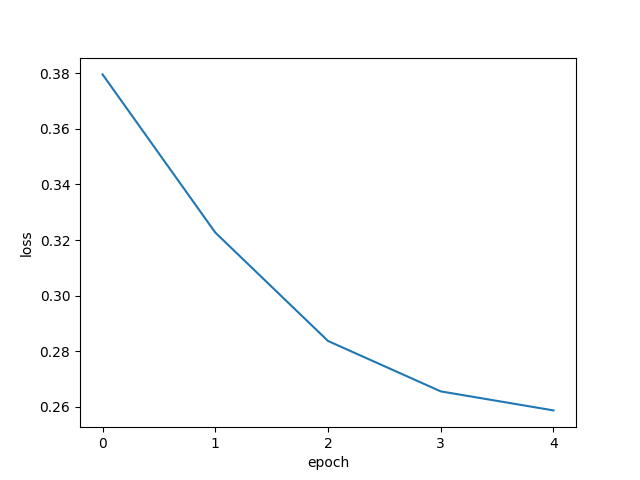
\includegraphics[width=0.5\textwidth]{graph.png}
\end{center}
\indent By applying gradient descent on the neural network, we adjust $C$ to minimize the loss, ideally converging to $C = 2.0$, thus correcting the error in the original function. Because the neural network is only an approximation of a program, the loss will never converge to zero even if the resulting hardened program becomes correct.

\section{Initial results}

At the time of writing We have made significant progress in the implementation of our programming language and neural net algorithms. The key components developed include:

\begin{itemize}
    \item \textbf{Language Parser}: We have implemented a parser that reads the custom programming language we designed for this project.

    \item \textbf{Abstract Syntax Tree (AST) and type checker}: The parser generates an typed checked AST representing the structure of the parsed programs.

    \item \textbf{Interpreter}: We have developed both a standard (hard) interpreter and a soft interpreter that evaluates the softened AST.

    \item \textbf{Softening Algorithm}: The algorithm replaces discrete operations with their soft counterparts in the AST.

    \item \textbf{Gradient and Backpropagation}: We have implemented gradient calculations and backpropagation to compute gradients of the loss function with respect to program parameters, allowing the training of our neural net.
\end{itemize}

Our current progress is summarized in the following checklist:

\begin{itemize}
    \item \textbf{Arithmetic Operations}:
    \begin{itemize}
        \item Addition: \Checkmark
        \item Subtraction: \Checkmark
        \item Multiplication: \Checkmark
        \item Division: \Checkmark
    \end{itemize}
    \item \textbf{Logical Operations}:
    \begin{itemize}
        \item Greater Than: \Checkmark
        \item Less Than: \Checkmark
        \item Not: \Checkmark
        \item Equality: Pending
        \item And, Or: Pending
    \end{itemize}
    \item \textbf{Control Flow}:
    \begin{itemize}
        \item If-Else Statements: \Checkmark
        \item For Loops: Pending
        \item While Loops: Pending
    \end{itemize}
    \item \textbf{Data Structures}:
    \begin{itemize}
        \item Lists: Pending
        \item Dictionaries: Pending
    \end{itemize}
\end{itemize}

We have tested our implementation on a few trivial sample programs and have observed results in correcting simple errors. For instance, in the example provided earlier, our neural net successfully adjusted the parameter $C$ from 3.0 to approximately 2.0, aligning the function's behavior with the expected outputs.

\section{Challenges}

During the development process, we encountered several challenges:

\begin{itemize}
    \item \textbf{Convergence Issues}: Convergence in the approximation space (the soft variant) does not always guarantee that the original discrete program will be correct after transformation. The behavior of the real program may still diverge from the desired output.

    \item \textbf{Non-Differentiability}: Not all operations remain double differentiable in their soft forms. This affects the calculation of second-order derivatives, limiting the use of advanced optimization methods like Newton's method, which requires the Hessian of the loss function.

    \item \textbf{Complex Control Flow and Data Structures}: Representing complex control flows like while loops and data structures like lists and dictionaries in a differentiable manner presents significant challenges.

    \item \textbf{Performance Considerations}: Currently, all computations are performed on the CPU. Scaling the system to handle larger programs efficiently may require moving computations to GPU using technologies like CUDA.
\end{itemize}

\section{Future Work}

Our next steps involve improving the efficiency, implementing more advance algorithsm from training our neural nets, and evaluating non-trivial code such as basic sorting algorithms.

\begin{itemize}
    \item \textbf{Complete Implementation of Basic Operations}: Finish implementing soft versions of all basic arithmetic and logical operations, including division, equality, and logical and/or. These operations should allow the language to be turing complete, and allow the neural net training of any valid program.

    \item \textbf{Implement Data Structures and Complex Control Flow}: Extend the system to support lists and dictionaries, including operations like getting, setting, and inserting elements. List will be implemented as a probility distribution, and dictionaries will use the self attention mechanism of the transformer model based off of a kernel function that should generalize to keys from any inner product space. Implement support of ``for'' and ``while'' loops. While loops may be approximated as infinitely long Markov chains to handle their potentially infinite nature. Fixed length for loops can be unrolled.

    \item \textbf{Synthetic Data Generation}: Automate the generation of test cases and incorrect program instances to evaluate the accuracy of the neural net representation's correction capabilities. We can do this generation by modifying the AST of a correct program to be correct, and use the correct program to generate many test cases based on random inputs.

    \item \textbf{Performance Optimization}: Explore the use of GPU acceleration to improve performance and scalability. We should translate our custom auto-differentiation framework to use Pytorch tensors to make the neural net training device independent. For more advanved programs the neural net may become very deep, up to thousands of layers requiring deep learning methods to be applied.

    \item \textbf{Testing on Non-Trivial Programs}: We also want to evaluate the correctness of the neural nets on more complicated programs. Our current testing consists only of trivial toy programs, we aim to test it on merge sort and bubble sort as our next steps.

    \item \textbf{More advanced training algorithsm}: We want to explore other training methods than just simple gradient descent. Based off the program parameters $W$ may be able to converge a lot faster by calculating the Hessian which scales $O(n^2)$ compared to the gradients scaling of $O(n)$ with respect to the number of parameters. For small programs this method may be able to converge more accurately and faster. Compared to gradient descent $W_{t+1} = W_t - \lambda \nabla L(W)$, we can use Newtons method to set the gradient to zero: $W_{t+1} = W_t - [\nabla^2 L(W_t)]^{-1}\nabla L(W_t)$.
\end{itemize}

\section{Conclusion}
We have made progress toward our goal of automating code correction by approximating imperative programs as neural networks. By developing a parser, AST, interpreters, and implementing soft versions of various operations, we have laid the groundwork for our system. Challenges remain, particularly in handling complex control flow and data structures, but we are optimistic about addressing these in future work. Our approach has the potential to significantly reduce the time and effort required for debugging and correcting code errors in software development.
\bibliographystyle{abbrv}
\bibliography{refs}
\end{document}
